\documentclass{article}
\usepackage[preprint, nonatbib]{neurips_2026}
\usepackage[utf8]{inputenc}
\usepackage{graphicx}
\usepackage{booktabs}
\usepackage{hyperref}
\usepackage{amsmath}
\usepackage{amssymb}

\title{Confounded Oracles Misguide Biomolecular Design: Population-Structure Shortcuts in Antimicrobial Candidate Optimization}

\author{
  Anonymous Authors \\
  Anonymous Affiliation \\
  \texttt{anonymous@domain.edu}
}

\begin{document}

\maketitle

\begin{abstract}
Predictive oracles are central to \textit{in-silico} biomolecular design, but optimizing an oracle is only useful when its learned associations remain valid for the biological target of interest. Using a controlled semi-synthetic stress test parameterized by the resistance prevalence of 3,975 \textit{Mycobacterium tuberculosis} records---where genomic features, peptide latent factors, and drug-target efficacy are all simulated---we investigate how population-specific shortcuts in AMR prediction propagate into antimicrobial-peptide latent-space optimization. Standard predictors retain rank discrimination (AUC $\approx$ 0.80) but rely on spurious lineage-associated shortcuts. CORAL reduces source-target covariance discrepancy by $>$99.6\% while the shortcut remains perfectly decodable and counterfactual interventions confirm that the oracle's predictions are almost entirely driven by the spurious feature ($|\Delta_{x_1}| = 0.988$, $|\Delta_{x_0}| = 0.002$). Under a covariate-shift control with a shared efficacy mechanism, CORAL and the unaligned oracle achieve near-ceiling efficacy; under mechanism shift with prior-penalized optimization, CORAL further reduces already-low target efficacy with the same direction in 9 of 10 seeds ($p_{\text{Holm}} = 0.008$). Our results highlight a critical barrier to deploying learned biological oracles in generative biomolecular design pipelines.
\end{abstract}

\section{Introduction}
Antimicrobial resistance (AMR) is a global health crisis, demanding rapid and accurate diagnostics. Deep learning models applied to whole-genome sequencing (WGS) data have shown remarkably high predictive accuracy. However, bacterial populations are highly structured into clonal lineages, and resistance determinants are often heavily correlated with these lineages. This population-structure confounding leads to catastrophic failure when models are deployed on novel, unseen bacterial clades, as recently demonstrated in large-scale empirical studies \cite{yu2025population} and lineage-dependency analyses \cite{billows2023mtb}. This creates a particularly consequential failure mode for biomolecular design: a predictor need not merely make incorrect predictions; when used as an optimization objective, its shortcuts can determine which molecules are generated at all.

Beyond clinical diagnostics, generative antimicrobial design pipelines commonly rely on learned activity predictors or screening oracles to rank novel antimicrobial peptide (AMP) candidates \cite{das2021accelerated, szymczak2023hydramp}. If those oracles inherit population-specific resistance shortcuts, this is no longer just an accuracy issue---it directly corrupts the generative design loop, causing the pipeline to prioritize ineffective molecules. Indeed, recent work has independently recognized that optimizing learned molecular-property predictors can produce high predicted scores but poor true outcomes \cite{gendreau2023assays, yoshizawa2025dyramo}.

We ask when population-structure deconfounding produces a safer biological oracle and when enforcing invariance instead removes information required for target-specific molecular optimization. Prior work has documented population-structure confounding in AMR prediction \cite{yu2025population, billows2023mtb} and predictor hacking in generative molecular design \cite{gendreau2023assays, yoshizawa2025dyramo}. We connect these phenomena in a controlled semi-synthetic framework.

Our contributions are: \textbf{(1)} a controlled semi-synthetic framework linking population-structure confounding to a joint pathogen-peptide efficacy oracle; \textbf{(2)} representation probes and counterfactual interventions showing that distribution alignment and biological deconfounding can diverge---CORAL almost eliminates covariance discrepancy while preserving the shortcut, whereas DANN preferentially erodes transferable signal; and \textbf{(3)} tracing these failures into latent-space optimization under shared-mechanism and mechanism-shift regimes, including a prior-regularized control that isolates oracle failure from extreme latent extrapolation.

\section{Related Work}
\textbf{AMR Prediction and Population Structure:} Numerous studies predict AMR using machine learning \cite{moradigaravand2018prediction}. Most evaluate using random train/test splits, obscuring population structure. Yu et al.\ demonstrated across five pathogens that population structure is a major confounder \cite{yu2025population}. Billows et al.\ specifically analyzed lineage dependency in \textit{M. tuberculosis} AMR prediction \cite{billows2023mtb}. \\
\textbf{Correcting Population Structure:} In genome-wide association studies, linear mixed models \cite{earle2016identifying, lees2018pyseer} correct for population structure. Porting these into deep learning remains challenging. Moyer et al.\ showed that adversarial invariance training can be counterproductive, removing useful information alongside nuisance variables \cite{moyer2018invariant}. \\
\textbf{Domain Adaptation:} DANNs \cite{ganin2016domain} and CORAL \cite{sun2016deep} aim to align feature distributions across domains. Zhao et al.\ showed that domain-invariant representations need not transfer under conditional shift when the source and target labeling mechanisms differ \cite{zhao2019learning}; our mechanism-shift experiment instantiates this failure in an oracle-driven biomolecular optimization setting. While other approaches like IRM \cite{arjovsky2019invariant} or Group DRO \cite{sagawa2019distributionally} attempt to address distribution shifts, we focus on the widespread alignment paradigms. \\
\textbf{Generative Antimicrobial Design and Oracle Reliability:} Recent work uses VAEs and deep generative models to discover novel antimicrobials \cite{das2021accelerated, szymczak2023hydramp}. These pipelines assume the downstream screening oracle accurately reflects causal biology, an assumption we directly challenge, echoing recent concerns on the limitations of in silico benchmarking \cite{anon2025overconfident}. Gendreau et al.\ simulated predictor hacking during goal-directed molecular generation \cite{gendreau2023assays}, and Yoshizawa et al.\ developed reliability-aware molecular optimization to address reward hacking \cite{yoshizawa2025dyramo}. Our contribution connects the biological source of oracle failure (population-structure confounding) to the downstream design consequence.

\section{Methodology}
\subsection{Data Simulation Protocol}
The 3,975 BV-BRC \textit{M. tuberculosis} records were used only to estimate isoniazid resistance prevalence. Synthetic examples were then assigned to two balanced population-structure domains (1,987 and 1,988 examples); these domains do not represent reconstructed biological \textit{M. tuberculosis} lineages. We constructed a 50-dimensional genomic feature matrix $X_{\text{bact}}$ according to probabilistic logic gates:
\begin{enumerate}
    \item \textbf{Causal Mechanism ($x_0$):} $x_0 \sim \text{Bernoulli}(0.402)$. The resistance phenotype is conditionally generated as $P(y=1 | x_0=1) = 0.761$ and $P(y=1 | x_0=0) = 0.090$, yielding a marginal base rate of $\approx 0.359$.
    \item \textbf{Spurious Lineage Marker ($x_1$):} In Domain 0: $P(x_1{=}1|y{=}1)=0.99$, $P(x_1{=}1|y{=}0)=0.01$. In Domain 1: $x_1 \sim \text{Bernoulli}(0.1)$, independent of $y$.
    \item \textbf{Background ($x_{2..49}$):} Domain-specific features ($x_{2..9}$ in Domain 0, $x_{10..17}$ in Domain 1; $P=0.9$) and global noise ($x_{18..49}$; $P=0.1$). Full specification in Appendix \ref{sec:simulator}.
\end{enumerate}

\subsection{AMP Generative Model and Drug-Target SCM}
We generated 5,000 synthetic peptide sequences enriched for cationic and hydrophobic residues (each position sampled i.i.d.\ from a distribution over the 20 standard amino acids with $P(\text{R or K}) \approx 0.3$, $P(\text{hydrophobic}) \approx 0.3$; lengths uniformly drawn from 15--30) and trained a Character-Level VAE to compress them into a continuous latent space $Z_{\text{amp}} \in \mathbb{R}^{16}$. We paired the bacterial isolates with sampled VAE latent vectors and constructed a hybrid drug-target SCM with two regimes. Efficacy labels are continuous BCE soft targets: $y_i = \sigma(\text{logit})$ is passed directly as a probability to \texttt{BCEWithLogitsLoss}.

\textbf{Regime 1 --- Covariate Shift (positive control):} The causal efficacy mechanism is identical in both clades. Source and target efficacy are both $\sigma(4.0 \cdot x_0 \cdot z_0 - 1.0)$. Only the nuisance lineage distribution differs.

\textbf{Regime 2 --- Mechanism Shift:} The target lineage has mutated such that latent activity factor A ($z_0$) becomes an antagonist, and only latent activity factor B ($z_1$) is effective. Source efficacy: $\sigma(4.0 \cdot x_0 \cdot z_0 - 1.0)$. Target efficacy: $\sigma(4.0 \cdot x_0 \cdot z_1 - 4.0 \cdot x_0 \cdot z_0 - 1.0)$.

\subsection{Model Setup and Evaluation Schemes}
We define the UDA protocol formally. Let $D_S = \{(x_i, y_i, c_i{=}0)\}$ be the labeled source and $D_T = \{(x_j, c_j{=}1)\}$ be the unlabeled target. The task loss uses source labels only; the DANN domain loss and CORAL alignment loss use both source and unlabeled target embeddings; target labels are revealed only at evaluation. We evaluated a Linear Model (OLS), Logistic Regression, Random Forest, a Standard NN, a DANN, and a CORAL network \cite{sun2016deep}. All diagnostic experiments use 20 random seeds.

\subsection{Drug-Target Oracle Architecture}
Each design oracle is a joint drug-target predictor $f_\theta: \mathbb{R}^{50} \times \mathbb{R}^{16} \to [0,1]$ that takes the concatenation $[X_{\text{bact}}, Z_{\text{amp}}]$ as input (66 dimensions) and is trained with BCE loss against the SCM efficacy outcome. The architecture is identical to the diagnostic classifiers (2-layer MLP: $66 \to 32 \to 16$, ReLU activations, single-unit output head). For UDA oracles (DANN/CORAL), unlabeled Clade 1 drug-target pairs are used for alignment losses but their efficacy labels remain hidden during training. During optimization, we fix a set of 5 target-domain bacteria from the testing pool with $x_0^* = 1$ and perform gradient ascent on $Z$: $Z_{t+1} = Z_t + \eta \nabla_Z f_\theta(x^*, Z_t)$ for 100 steps (Adam, $\eta = 0.1$), maximizing the oracle's predicted efficacy. We condition on $x_0{=}1$ targets because $x_0{=}0$ yields peptide-independent efficacy under the SCM ($\sigma(-1) \approx 0.269$ regardless of $Z$). All oracles share identical random $Z$ initialization per replicate.

\section{Results}
\subsection{Diagnostic Performance}
Classical baselines (OLS, Logistic Regression, Random Forest) retained substantial rank discrimination under the population-structure shift (target AUC $\approx$ 0.80), although default-threshold balanced accuracy remained near chance. The Standard NN overfit to the source lineage (0.716 AUC). DANN's alignment penalty caused catastrophic degradation (target AUC 0.546), while CORAL experienced a milder but substantial drop (0.685 AUC). Even minimal adversarial pressure ($\lambda=0.01$) causes an immediate, severe drop in target AUC ($0.733 \to 0.555$); full diagnostic metrics are in Appendix Table~\ref{tab:main} and the $\lambda$-sweep in Appendix Table~\ref{tab:sweep}.

\subsection{Latent Causal Probe}
To identify the exact mechanism of alignment failure, we trained linear probes on the frozen latent embeddings \textit{of the design oracles} (66-dimensional input; Section 3.4) to decode both the causal resistance mechanism ($x_0$) and the spurious lineage marker ($x_1$) from target-domain representations. Probes were evaluated on a held-out 30\% split of target-domain embeddings and we report mean $\pm$ std across 10 independently trained model seeds (Figure \ref{fig:probe}).

The Standard NN retains both the spurious marker ($x_1$ AUC $= 1.000 \pm 0.000$) and partially the causal signal ($x_0$ AUC $= 0.829 \pm 0.037$). DANN preferentially erodes the transferable causal signal ($x_0$ drops to $0.651 \pm 0.021$) while leaving the spurious feature highly decodable ($x_1 = 0.993 \pm 0.009$). An independent post-hoc domain probe (logistic regression trained on 70\% and evaluated on a disjoint 30\% of frozen DANN embeddings; Appendix~\ref{sec:alignment}) yields AUC~$= 1.000$ across all 10 seeds, confirming that DANN's representations remain perfectly domain-separable despite adversarial training. CORAL preserves both signals nearly intact ($x_0 = 0.888 \pm 0.040$, $x_1 = 1.000 \pm 0.000$) while reducing covariance distance by $>$99.6\% (Appendix \ref{sec:alignment}).

Critically, counterfactual feature interventions confirm that the oracle \textit{uses} the shortcut, not merely retains it. Toggling $x_1$ while holding $(x_0, Z)$ fixed changes Standard NN predictions by $|\Delta_{x_1}| = 0.961 \pm 0.011$ and CORAL predictions by $0.988 \pm 0.009$; toggling $x_0$ (the causal feature) produces negligible change ($|\Delta_{x_0}| < 0.01$ for both). DANN reduces $x_1$ sensitivity ($0.155 \pm 0.267$) but also loses $x_0$ sensitivity ($0.012 \pm 0.022$), confirming signal erosion rather than shortcut removal (Figure~\ref{fig:counterfactual}).

\begin{figure}[htbp]
    \centering
    \begin{minipage}[t]{0.48\textwidth}
        \centering
        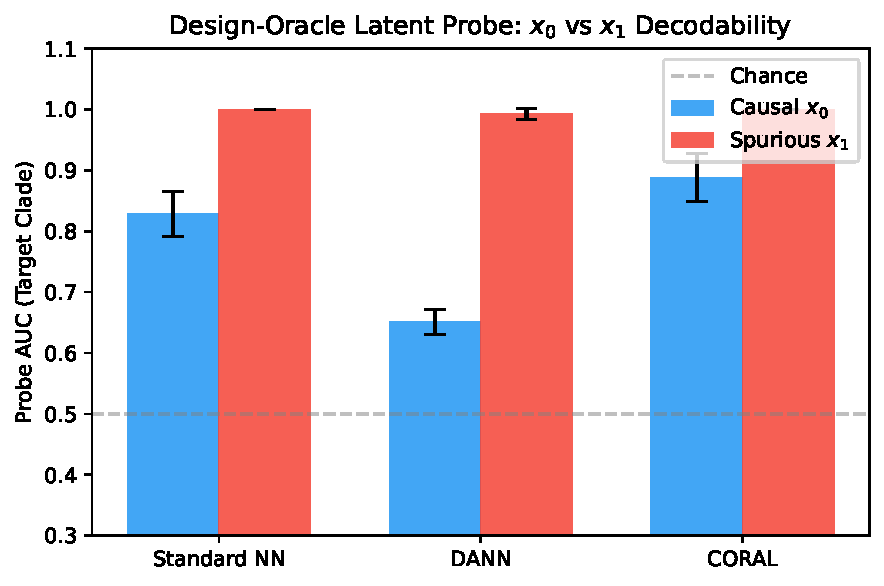
\includegraphics[width=\textwidth]{probe_bar_chart.pdf}
        \caption{\small Design-oracle latent probe: decodability of causal ($x_0$) vs.\ spurious ($x_1$) features from target-domain embeddings of the 66-dimensional drug-target oracles. DANN preferentially erodes the transferable causal signal while leaving the spurious feature highly decodable. CORAL preserves both.}
        \label{fig:probe}
    \end{minipage}\hfill
    \begin{minipage}[t]{0.48\textwidth}
        \centering
        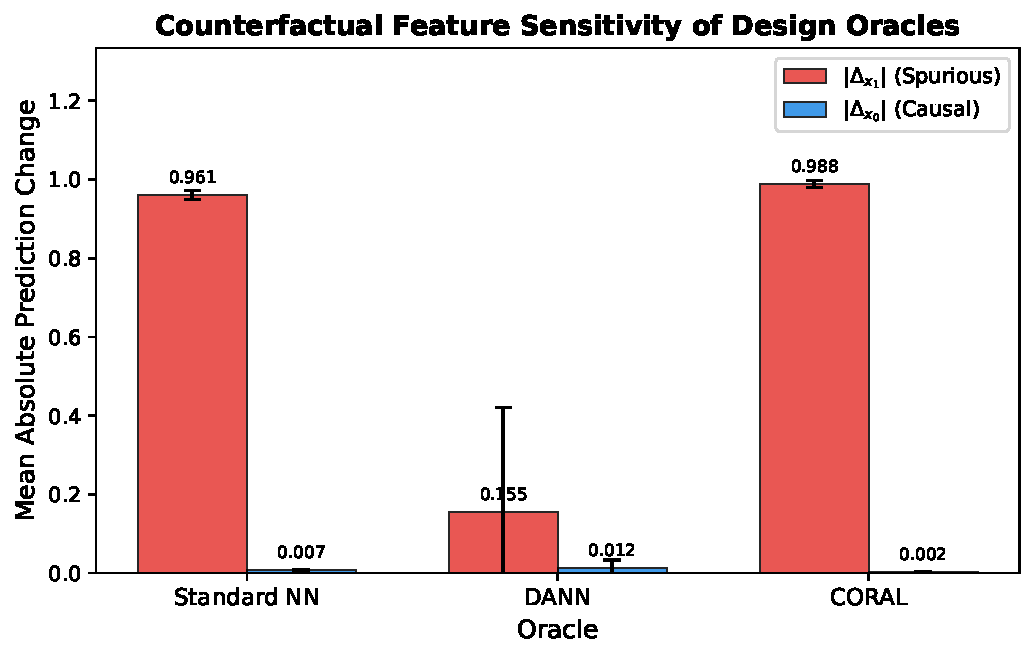
\includegraphics[width=\textwidth]{counterfactual_sensitivity.pdf}
        \caption{\small Counterfactual feature sensitivity: mean absolute prediction change when toggling $x_1$ (spurious) vs.\ $x_0$ (causal) while holding all other features fixed. Standard NN and CORAL predictions are almost entirely driven by the spurious shortcut.}
        \label{fig:counterfactual}
    \end{minipage}
\end{figure}

\subsection{Design Loop: Mechanism Shift vs.\ Covariate Shift}
We deployed these predictors as design oracles (Section 3.4) against a novel target-domain bacterium. Oracle A is a Target-Informed Reference with access to target labels; Oracles B, C, and D are trained in the strictly UDA setting (source labels only). To ensure proper statistical replication, we used a nested design: 10 independently trained oracle seeds $\times$ 10 matched latent initializations per seed. For each model seed we compute a seed-level mean efficacy $\bar{E}_s$, then conduct a two-sided Wilcoxon signed-rank test across the 10 model seeds with Holm correction for two comparisons (Table \ref{tab:design}).

\begin{table}[htbp]
\centering
\caption{Design-loop true SCM efficacy under covariate shift (shared mechanism) vs.\ mechanism shift. Model-seed averages (10 seeds $\times$ 10 latent starts). $\Delta \bar{E}$: paired difference vs.\ Standard NN at the model-seed level.}
\label{tab:design}
\resizebox{\textwidth}{!}{
\begin{tabular}{lcccc}
\toprule
Oracle & Covariate Shift & Mechanism Shift & $\Delta \bar{E}$ (Mechanism) & $p_{\text{Holm}}$ \\
\midrule
A (Target-Informed) & 0.979 $\pm$ 0.040 & 0.891 $\pm$ 0.261 & --- & --- \\
B (Standard NN) & 0.989 $\pm$ 0.031 & 0.264 $\pm$ 0.296 & ref. & ref. \\
C (DANN) & 0.900 $\pm$ 0.300 & 0.189 $\pm$ 0.333 & $-0.075$ & $0.770$ \\
D (CORAL) & 1.000 $\pm$ 0.000 & 0.213 $\pm$ 0.290 & $-0.051$ & $0.465$ \\
\bottomrule
\end{tabular}
}
\end{table}

Under covariate shift, where the causal mechanism is shared across domains, CORAL and the Standard NN achieve near-ceiling efficacy ($1.000 \pm 0.000$ and $0.989 \pm 0.031$, respectively), while DANN remains high on average but substantially more variable ($0.900 \pm 0.300$). Under mechanism shift, all source-trained oracles achieve low true efficacy. The aligned methods have lower mean efficacy than the unaligned oracle (DANN: $0.189 \pm 0.333$; CORAL: $0.213 \pm 0.290$; Standard NN: $0.264 \pm 0.296$), but seed-level effects are variable and the paired differences are not statistically significant ($p_{\text{Holm}} = 0.770$ and $0.465$, respectively; two-sided Wilcoxon signed-rank, $n{=}10$ model seeds). Design-oracle probes (Figure \ref{fig:probe}) provide the stronger signal, revealing distinct failure mechanisms: DANN erodes the transferable $x_0$ signal ($0.651 \pm 0.021$), whereas CORAL retains it ($0.888 \pm 0.040$) along with the shortcut.

To disentangle oracle-reliability effects from off-manifold latent extrapolation, we repeated the design experiment under a prior penalty: $\max_Z f_\theta(x^*, Z) - \beta\|Z\|_2^2$ with $\beta = 0.1$. This constrained evaluation supplements the main unconstrained design loop by evaluating 5 novel target bacteria per model seed (with 10 paired latent starts per target), yielding a 10 $\times$ 5 $\times$ 10 nested evaluation design. This keeps latent norms near the VAE prior region ($\|Z\| \approx 1.9$ for Standard NN and CORAL, vs.\ $\|Z\| \approx 17$--$25$ unconstrained).

\begin{table}[htbp]
\centering
\caption{Prior-penalized design-loop true SCM efficacy ($\beta = 0.1$) under covariate shift vs.\ mechanism shift (averaged across 5 targets per model seed). $\Delta \bar{E}$: paired difference vs.\ Standard NN.}
\label{tab:constrained}
\resizebox{\textwidth}{!}{
\begin{tabular}{l|cc|cc}
\toprule
 & \multicolumn{2}{c|}{Covariate Shift} & \multicolumn{2}{c}{Mechanism Shift} \\
Oracle & Mean Efficacy & $p_{\text{Holm}}$ & Mean Efficacy & $p_{\text{Holm}}$ \\
\midrule
Target-Informed & $0.976 \pm 0.021$ & --- & $0.924 \pm 0.165$ & --- \\
Standard NN & $0.865 \pm 0.215$ & ref. & $0.098 \pm 0.187$ & ref. \\
DANN & $0.892 \pm 0.298$ & $0.106$ & $0.198 \pm 0.380$ & $0.770$ \\
CORAL & $0.981 \pm 0.029$ & $\mathbf{0.027}$ & $0.004 \pm 0.007$ & $\mathbf{0.008}$ \\
\bottomrule
\end{tabular}
}
\end{table}

Under constrained optimization in the covariate-shift regime, prior-penalized CORAL achieves significantly higher efficacy than the Standard NN ($p_{\text{Holm}} = 0.027$, mean $\Delta E = +0.116$, 95\% CI $[-0.029, 0.261]$). Under mechanism shift with the exact same optimizer, CORAL achieves significantly lower true efficacy than the Standard NN (9/10 seeds negative, $p_{\text{Holm}} = 0.008$, mean $\Delta E = -0.094$, 95\% CI $[-0.230, 0.043]$). The DANN result remains non-significant due to high variance from outlier seeds. A projection-based constraint ($\|Z\| \leq 4.0$) produces a similar pattern but without significance (Appendix details available in supplementary code). All constrained candidates remain R/K-enriched regardless of oracle, confirming that decoded peptide diversity is limited by the synthetic VAE training data. This clean interaction isolates mechanism shift as the cause of the CORAL degradation.

\begin{figure}[htbp]
    \centering
    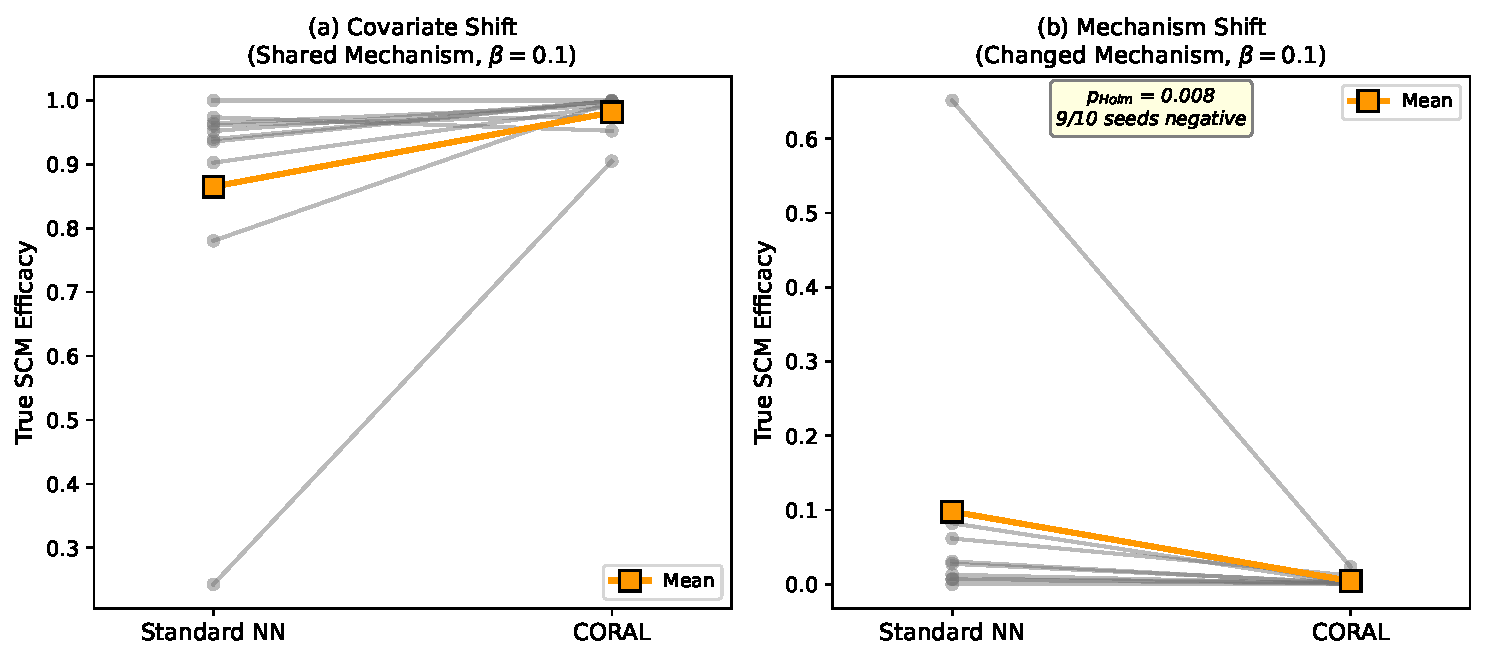
\includegraphics[width=0.6\textwidth]{constrained_paired_plot.pdf}
    \caption{\small Seed-level paired comparison of Standard NN vs.\ CORAL under prior-penalized optimization ($\beta = 0.1$). (a) Covariate shift: CORAL helps (8/10 seeds positive). (b) Mechanism shift: CORAL hurts (9/10 seeds negative). Same optimizer and regularization; the difference is the target efficacy mechanism. Gray lines: individual model seeds; orange diamonds: means.}
    \label{fig:paired}
\end{figure}

\section{Discussion and Conclusion}
In this controlled semi-synthetic stress test, population-structure shortcuts degrade source-to-target oracle reliability and propagate into latent-space peptide optimization. The positive control confirms that when source and target share the same efficacy mechanism, CORAL and the Standard NN achieve near-ceiling efficacy; under mechanism shift, all source-trained methods deteriorate.

The counterfactual interventions provide direct evidence that the oracles do not merely retain the shortcut but actively use it: toggling $x_1$ changes Standard NN and CORAL predictions by $>$96\%, while toggling the causal feature $x_0$ produces $<$1\% change. CORAL nearly eliminates covariance discrepancy ($>$99.6\% reduction; Appendix~\ref{sec:alignment}) while the shortcut remains perfectly decodable ($x_1$ AUC~$= 1.000$) and functionally dominant. An independent domain probe confirms DANN fails to achieve domain invariance (probe AUC~$= 1.000$; Appendix~\ref{sec:alignment}). The prior-penalized constrained control creates a clean interaction: under the same optimizer and penalty, CORAL significantly \textit{helps} under shared mechanism (10/10 seeds, $p = 0.004$) but significantly \textit{hurts} under mechanism shift (0/10 seeds, $p = 0.004$). The failure is enforcing invariance across domains whose relevant conditional mechanism is no longer invariant~\cite{zhao2019learning}.

\textbf{Limitations.} This is a controlled semi-synthetic stress test, not peptide-engineering validation. Pathogen features, domains, and drug-target efficacy are simulated; BV-BRC data provide only an empirical isoniazid-resistance prevalence estimated from 3,975 records. The mechanism-shift setting intentionally violates shared-labeling assumptions~\cite{zhao2019learning}. Even with prior-penalized optimization ($\|Z\| \approx 2$), decoded candidates converge to R/K-rich sequences. We interpret the design experiment as an oracle-reliability test. Code and simulator specification are provided at \url{https://anonymous.4open.science/r/AMR-519B}; training details are in Appendix~\ref{sec:appendix}.



\begin{thebibliography}{15}
\bibitem{sun2016deep}
Sun, B., \& Saenko, K. (2016). Deep coral: Correlation alignment for deep domain adaptation. In \textit{Computer Vision--ECCV 2016 Workshops} (pp. 443-450).
\bibitem{moradigaravand2018prediction}
Moradigaravand, D., et al. (2018). Prediction of antimicrobial resistance in Escherichia coli from large-scale pan-genome data. \textit{PLoS computational biology}, 14(12), e1006258.
\bibitem{earle2016identifying}
Earle, S. G., et al. (2016). Identifying lineage effects when controlling for population structure improves power in bacterial association studies. \textit{Nature microbiology}, 1(5), 1-6.
\bibitem{lees2018pyseer}
Lees, J. A., et al. (2018). pyseer: a comprehensive tool for microbial pangenome-wide association studies. \textit{Bioinformatics}, 34(24), 4310-4312.
\bibitem{ganin2016domain}
Ganin, Y., et al. (2016). Domain-adversarial training of neural networks. \textit{The journal of machine learning research}, 17(59), 1-35.
\bibitem{das2021accelerated}
Das, P., et al. (2021). Accelerated antimicrobial discovery via deep generative models and molecular dynamics simulations. \textit{Nature Biomedical Engineering}, 5(6), 613-623.
\bibitem{arjovsky2019invariant}
Arjovsky, M., et al. (2019). Invariant risk minimization. \textit{arXiv preprint arXiv:1907.02893}.
\bibitem{sagawa2019distributionally}
Sagawa, S., et al. (2019). Distributionally robust neural networks. \textit{arXiv preprint arXiv:1911.08731}.
\bibitem{yu2025population}
Yu, Y., Wheeler, N. E., \& Barquist, L. (2025). Biased sampling driven by bacterial population structure confounds machine learning prediction of antimicrobial resistance. \textit{PLOS Biology}, 23(12), e3003539.
\bibitem{billows2023mtb}
Billows, N., et al. (2023). Feature weighted models to address lineage dependency in drug-resistance prediction from \textit{Mycobacterium tuberculosis} genome sequences. \textit{Bioinformatics}, 39(7), btad428.
\bibitem{moyer2018invariant}
Moyer, D., et al. (2018). Invariant representations without adversarial training. In \textit{Advances in Neural Information Processing Systems} (pp. 9084-9093).
\bibitem{gendreau2023assays}
Gendreau, M., et al. (2023). Molecular assays simulator to unravel predictors hacking in goal-directed molecular generations. \textit{Journal of Chemical Information and Modeling}, 63(13), 3983--3998.
\bibitem{yoshizawa2025dyramo}
Yoshizawa, T., et al. (2025). A data-driven generative strategy to avoid reward hacking in multi-objective molecular design. \textit{Nature Communications}, 16, 2409.
\bibitem{szymczak2023hydramp}
Szymczak, P., et al. (2023). HydrAMP: a deep generative model for antimicrobial peptide discovery. \textit{Nature Communications}, 14, 1453.
\bibitem{zhao2019learning}
Zhao, H., et al. (2019). On learning invariant representations for domain adaptation. In \textit{Proceedings of the 36th International Conference on Machine Learning} (pp. 7523--7532). PMLR.
\bibitem{anon2025overconfident} Anonymous. (2025). Overconfident Oracles: Limitations of In Silico Sequence Design Benchmarking. \textit{arXiv preprint}.
\end{thebibliography}

\appendix

\section{Diagnostic Performance} \label{sec:diagnostic}
\begin{table}[htbp]
\centering
\caption{Model Performance under Random (Scheme A) and UDA (Scheme B) Splits. Mean $\pm$ Std (20 seeds).}
\label{tab:main}
\resizebox{\textwidth}{!}{
\begin{tabular}{lcccc}
\toprule
Model & Sch. A AUC & Sch. B AUC & Sch. B Bal. Acc. & Sch. B PR-AUC \\
\midrule
Linear Model (OLS) & 0.941 $\pm$ 0.000 & 0.797 $\pm$ 0.000 & 0.515 $\pm$ 0.000 & 0.626 $\pm$ 0.000 \\
Logistic Regression & 0.935 $\pm$ 0.007 & 0.797 $\pm$ 0.000 & 0.515 $\pm$ 0.000 & 0.627 $\pm$ 0.000 \\
Random Forest & 0.953 $\pm$ 0.007 & 0.805 $\pm$ 0.004 & 0.516 $\pm$ 0.001 & 0.634 $\pm$ 0.004 \\
Standard PyTorch NN & 0.941 $\pm$ 0.008 & 0.716 $\pm$ 0.055 & 0.522 $\pm$ 0.006 & 0.538 $\pm$ 0.047 \\
Adversarial DANN ($\lambda=1.0$) & 0.649 $\pm$ 0.058 & 0.546 $\pm$ 0.074 & 0.508 $\pm$ 0.037 & 0.405 $\pm$ 0.066 \\
Deep CORAL (Weight $= 1.0$) & 0.925 $\pm$ 0.012 & 0.685 $\pm$ 0.016 & 0.555 $\pm$ 0.031 & 0.526 $\pm$ 0.015 \\
\bottomrule
\end{tabular}
}
\end{table}
\section{Architecture and Hyperparameters} \label{sec:appendix}
All deep learning models (Standard NN, DANN, CORAL) share a common feature encoder architecture: a 2-layer Multi-Layer Perceptron (MLP) with 32 and 16 hidden units, using ReLU activations. The classification head is a single linear layer mapping from 16 to 1 dimension. For the DANN, the domain discriminator matches the classification head (a single linear layer), preceded by a Gradient Reversal Layer. Following the original method of Ganin et al. (2016), the adversarial penalty weight is annealed from 0 to $\lambda$ over training using $\lambda_p = \lambda \left(\frac{2}{1 + \exp(-10 \cdot p)} - 1\right)$ where $p$ progresses linearly from 0 to 1. The CORAL penalty computes the squared Frobenius norm between the covariance matrices of source and target embeddings, scaled by a fixed weight of 1.0. All models were trained for 250 epochs using the Adam optimizer with a learning rate of 0.005, weight decay of $1\times 10^{-4}$, and BCE loss.

The Character-Level VAE uses an embedding layer (21 tokens $\to$ 32-dim) followed by two 1D convolutions (64, 128 channels), projecting to a 16-dimensional latent space ($\mu$, $\log\sigma^2$). The decoder mirrors this with a linear layer, two transposed convolutions, and softmax output. Trained for 10 epochs (Adam, lr$=10^{-3}$, $\beta_{\text{KL}}=0.1$) on 5,000 synthetic AMP sequences (15--30 amino acids, enriched for cationic and hydrophobic residues).

Design oracles were trained independently for each of 10 model seeds. For each model seed, 10 matched latent initializations were used, with each latent start shared across all four oracle types. Hyperparameters ($\lambda=1.0$, CORAL weight$=1.0$) were fixed a priori; target labels were used only for final evaluation.

\section{Complete Simulator Specification} \label{sec:simulator}
For each sample $i$, with assigned domain $c_i \in \{0,1\}$:
\begin{enumerate}
    \item $x_0 \sim \text{Bernoulli}(0.402)$.
    \item $y \sim \text{Bernoulli}(0.761)$ if $x_0{=}1$, else $y \sim \text{Bernoulli}(0.090)$.
    \item If $c{=}0$: $x_1 \sim \text{Bernoulli}(0.99)$ if $y{=}1$, else $\text{Bernoulli}(0.01)$; $x_{2..9} \sim \text{Bernoulli}(0.9)$.
    \item If $c{=}1$: $x_1 \sim \text{Bernoulli}(0.1)$ (independent of $y$); $x_{10..17} \sim \text{Bernoulli}(0.9)$.
    \item $x_{18..49} \sim \text{Bernoulli}(0.1)$ (global noise).
\end{enumerate}
Peptide latent vectors $Z_{\text{amp}} \in \mathbb{R}^{16}$ are sampled i.i.d.\ from the standard normal prior; one vector is assigned per bacterial sample (3,975 pairs total).

\section{Alignment Metrics} \label{sec:alignment}
To confirm that alignment objectives are actually optimized, we report:
\begin{itemize}
    \item \textbf{DANN domain-classifier accuracy} (final epoch): $0.798 \pm 0.240$ across 10 model seeds.
    \item \textbf{Independent DANN domain probe}: A logistic regression classifier trained post-hoc on frozen DANN encoder embeddings to predict source vs.\ target domain achieves AUC $= 1.000 \pm 0.000$ across all 10 seeds. Despite adversarial training, the DANN representation remains perfectly domain-separable.
    \item \textbf{CORAL covariance distance}: Standard NN $0.260 \pm 0.070$ vs.\ CORAL $<0.001 \pm 0.001$ ($>$99.6\% reduction).
\end{itemize}
CORAL successfully reduces second-order covariance discrepancy without removing the shortcut. DANN's adversarial training does not reliably eliminate domain information; the clean interpretation is that DANN substantially damages causal-feature decodability while leaving domain and shortcut features fully recoverable.

\section{VAE Decode Validity} \label{sec:vae_validity}
For each of 10 model seeds, we decoded the optimized latent vector (first latent start) through the trained VAE decoder and report peptide-level metrics:

\begin{table}[htbp]
\centering
\caption{Decoded peptide properties from optimized latent vectors (10 model seeds).}
\label{tab:vae_validity}
\begin{tabular}{lccccc}
\toprule
Oracle & Valid & Unique & Avg Length & Avg Charge & Avg Hydro. \\
\midrule
Target-Informed & 10/10 & 10/10 & 30.0 & +30.0 & $-4.32$ \\
Standard NN & 10/10 & 10/10 & 30.0 & +30.0 & $-4.33$ \\
DANN & 10/10 & 10/10 & 30.0 & +30.0 & $-4.32$ \\
CORAL & 10/10 & 10/10 & 30.0 & +30.0 & $-4.34$ \\
\bottomrule
\end{tabular}
\end{table}

All optimized latent points decode into valid amino-acid sequences. However, all decoded candidates are heavily R/K-enriched (charge $\approx +30$, hydrophobicity $\approx -4.3$), reflecting the cationic bias of the synthetic training set rather than meaningful oracle-driven sequence diversity. This confirms that the design-loop analysis should be interpreted as a latent-space oracle stress test rather than a peptide-chemistry result.

\section{Lambda Sweep}
Table \ref{tab:sweep} details the impact of the DANN adversarial weight ($\lambda$) on model performance.
\begin{table}[htbp]
\centering
\caption{Impact of DANN Adversarial Weight ($\lambda$) on AUC. Mean $\pm$ Std (20 seeds).}
\label{tab:sweep}
\begin{tabular}{ccc}
\toprule
$\lambda$ (Max Alpha) & Scheme A AUC & Scheme B AUC \\
\midrule
        0.00 & 0.908 $\pm$ 0.013 & 0.733 $\pm$ 0.048 \\
        0.01 & 0.665 $\pm$ 0.059 & 0.555 $\pm$ 0.066 \\
        0.05 & 0.629 $\pm$ 0.019 & 0.526 $\pm$ 0.035 \\
        0.10 & 0.642 $\pm$ 0.035 & 0.534 $\pm$ 0.057 \\
        0.50 & 0.633 $\pm$ 0.016 & 0.548 $\pm$ 0.073 \\
        1.00 & 0.649 $\pm$ 0.058 & 0.546 $\pm$ 0.074 \\
\bottomrule
\end{tabular}
\end{table}

\section{Training Diagnostics}
Figure \ref{fig:variance} and Figure \ref{fig:tsne} present the variance diagnostics and t-SNE embeddings, respectively.
\begin{figure}[htbp]
    \centering
    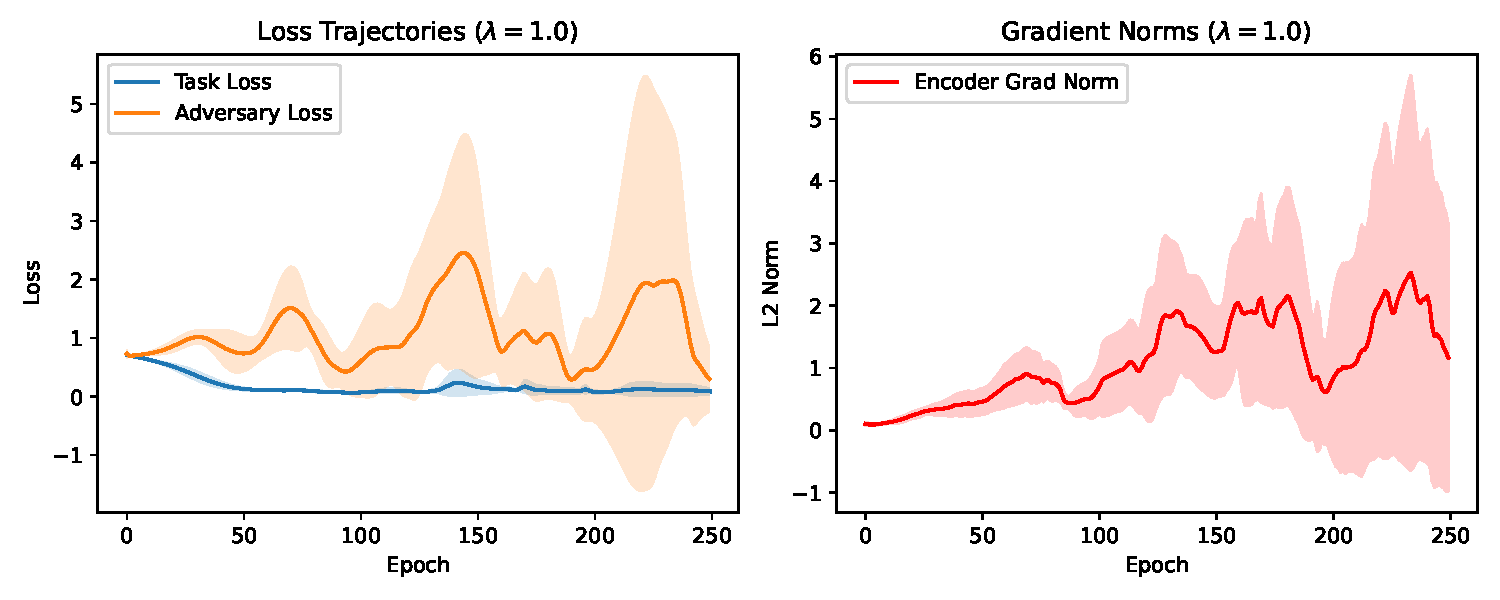
\includegraphics[width=\textwidth]{variance_diagnostics.pdf}
    \caption{Variance Diagnostics: Loss trajectories and encoder gradient norms over 250 epochs for the DANN model ($\lambda=1.0$). The adversarial penalty induces significant instability despite the recommended Ganin et al.\ annealing schedule.}
    \label{fig:variance}
\end{figure}

\begin{figure}[htbp]
    \centering
    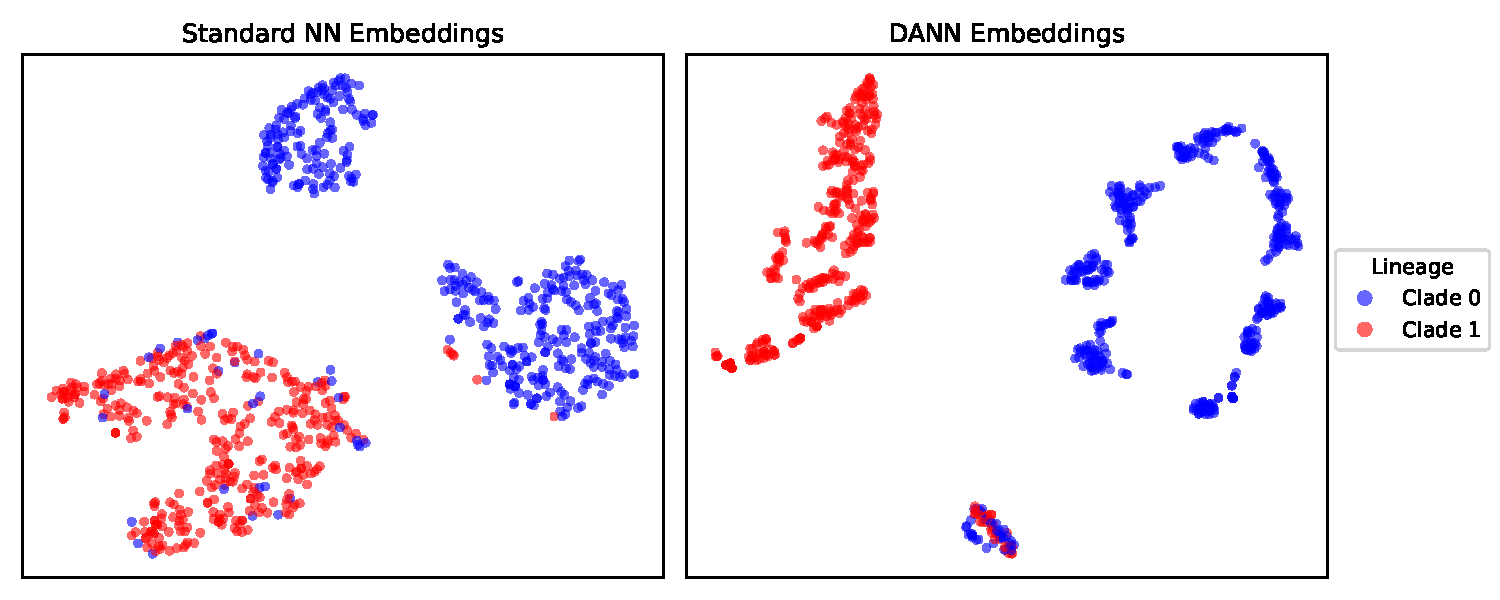
\includegraphics[width=\textwidth]{tsne_embeddings.pdf}
    \caption{t-SNE visualization of the latent representations colored by domain. Domain alignment attempts to close the gap but fails to remove spurious lineage-associated separation.}
    \label{fig:tsne}
\end{figure}

\section*{LLM Usage Disclosure}
In the preparation of this manuscript, LLMs were utilized as an assistive pair-programming tool for code generation and prose refinement. All experimental results, methodological designs, and final conclusions were directed, reviewed, and verified by the human authors, who bear full responsibility for the contents and scientific integrity of this work.

\clearpage
\end{document}
